
%% bare_conf.tex
%% V1.3
%% 2007/01/11
%% by Michael Shell
%% See:
%% http://www.michaelshell.org/
%% for current contact information.
%%
%% This is a skeleton file demonstrating the use of IEEEtran.cls
%% (requires IEEEtran.cls version 1.7 or later) with an IEEE conference paper.
%%
%% Support sites:
%% http://www.michaelshell.org/tex/ieeetran/
%% http://www.ctan.org/tex-archive/macros/latex/contrib/IEEEtran/
%% and
%% http://www.ieee.org/

%%*************************************************************************
%% Legal Notice:
%% This code is offered as-is without any warranty either expressed or
%% implied; without even the implied warranty of MERCHANTABILITY or
%% FITNESS FOR A PARTICULAR PURPOSE! 
%% User assumes all risk.
%% In no event shall IEEE or any contributor to this code be liable for
%% any damages or losses, including, but not limited to, incidental,
%% consequential, or any other damages, resulting from the use or misuse
%% of any information contained here.
%%
%% All comments are the opinions of their respective authors and are not
%% necessarily endorsed by the IEEE.
%%
%% This work is distributed under the LaTeX Project Public License (LPPL)
%% ( http://www.latex-project.org/ ) version 1.3, and may be freely used,
%% distributed and modified. A copy of the LPPL, version 1.3, is included
%% in the base LaTeX documentation of all distributions of LaTeX released
%% 2003/12/01 or later.
%% Retain all contribution notices and credits.
%% ** Modified files should be clearly indicated as such, including  **
%% ** renaming them and changing author support contact information. **
%%
%% File list of work: IEEEtran.cls, IEEEtran_HOWTO.pdf, bare_adv.tex,
%%                    bare_conf.tex, bare_jrnl.tex, bare_jrnl_compsoc.tex
%%*************************************************************************

% *** Authors should verify (and, if needed, correct) their LaTeX system  ***
% *** with the testflow diagnostic prior to trusting their LaTeX platform ***
% *** with production work. IEEE's font choices can trigger bugs that do  ***
% *** not appear when using other class files.                            ***
% The testflow support page is at:
% http://www.michaelshell.org/tex/testflow/



% Note that the a4paper option is mainly intended so that authors in
% countries using A4 can easily print to A4 and see how their papers will
% look in print - the typesetting of the document will not typically be
% affected with changes in paper size (but the bottom and side margins will).
% Use the testflow package mentioned above to verify correct handling of
% both paper sizes by the user's LaTeX system.
%
% Also note that the "draftcls" or "draftclsnofoot", not "draft", option
% should be used if it is desired that the figures are to be displayed in
% draft mode.
%
\documentclass[conference]{IEEEtran}
% Add the compsoc option for Computer Society conferences.
%
% If IEEEtran.cls has not been installed into the LaTeX system files,
% manually specify the path to it like:
% \documentclass[conference]{../sty/IEEEtran}





% Some very useful LaTeX packages include:
% (uncomment the ones you want to load)


% *** MISC UTILITY PACKAGES ***
%
%\usepackage{ifpdf}
% Heiko Oberdiek's ifpdf.sty is very useful if you need conditional
% compilation based on whether the output is pdf or dvi.
% usage:
% \ifpdf
%   % pdf code
% \else
%   % dvi code
% \fi
% The latest version of ifpdf.sty can be obtained from:
% http://www.ctan.org/tex-archive/macros/latex/contrib/oberdiek/
% Also, note that IEEEtran.cls V1.7 and later provides a builtin
% \ifCLASSINFOpdf conditional that works the same way.
% When switching from latex to pdflatex and vice-versa, the compiler may
% have to be run twice to clear warning/error messages.

%used for symbols
\usepackage{gensymb}




% *** CITATION PACKAGES ***
%
\usepackage{cite}
% cite.sty was written by Donald Arseneau
% V1.6 and later of IEEEtran pre-defines the format of the cite.sty package
% \cite{} output to follow that of IEEE. Loading the cite package will
% result in citation numbers being automatically sorted and properly
% "compressed/ranged". e.g., [1], [9], [2], [7], [5], [6] without using
% cite.sty will become [1], [2], [5]--[7], [9] using cite.sty. cite.sty's
% \cite will automatically add leading space, if needed. Use cite.sty's
% noadjust option (cite.sty V3.8 and later) if you want to turn this off.
% cite.sty is already installed on most LaTeX systems. Be sure and use
% version 4.0 (2003-05-27) and later if using hyperref.sty. cite.sty does
% not currently provide for hyperlinked citations.
% The latest version can be obtained at:
% http://www.ctan.org/tex-archive/macros/latex/contrib/cite/
% The documentation is contained in the cite.sty file itself.






% *** GRAPHICS RELATED PACKAGES ***
%
\ifCLASSINFOpdf
  \usepackage[pdftex]{graphicx}
  % declare the path(s) where your graphic files are
  \graphicspath{figures}
  % and their extensions so you won't have to specify these with
  % every instance of \includegraphics
  \DeclareGraphicsExtensions{.pdf,.jpeg,.png}
\else
  % or other class option (dvipsone, dvipdf, if not using dvips). graphicx
  % will default to the driver specified in the system graphics.cfg if no
  % driver is specified.
  % \usepackage[dvips]{graphicx}
  % declare the path(s) where your graphic files are
  % \graphicspath{{../eps/}}
  % and their extensions so you won't have to specify these with
  % every instance of \includegraphics
  % \DeclareGraphicsExtensions{.eps}
\fi
% graphicx was written by David Carlisle and Sebastian Rahtz. It is
% required if you want graphics, photos, etc. graphicx.sty is already
% installed on most LaTeX systems. The latest version and documentation can
% be obtained at: 
% http://www.ctan.org/tex-archive/macros/latex/required/graphics/
% Another good source of documentation is "Using Imported Graphics in
% LaTeX2e" by Keith Reckdahl which can be found as epslatex.ps or
% epslatex.pdf at: http://www.ctan.org/tex-archive/info/
%
% latex, and pdflatex in dvi mode, support graphics in encapsulated
% postscript (.eps) format. pdflatex in pdf mode supports graphics
% in .pdf, .jpeg, .png and .mps (metapost) formats. Users should ensure
% that all non-photo figures use a vector format (.eps, .pdf, .mps) and
% not a bitmapped formats (.jpeg, .png). IEEE frowns on bitmapped formats
% which can result in "jaggedy"/blurry rendering of lines and letters as
% well as large increases in file sizes.
%
% You can find documentation about the pdfTeX application at:
% http://www.tug.org/applications/pdftex





% *** MATH PACKAGES ***
%
%\usepackage[cmex10]{amsmath}
% A popular package from the American Mathematical Society that provides
% many useful and powerful commands for dealing with mathematics. If using
% it, be sure to load this package with the cmex10 option to ensure that
% only type 1 fonts will utilized at all point sizes. Without this option,
% it is possible that some math symbols, particularly those within
% footnotes, will be rendered in bitmap form which will result in a
% document that can not be IEEE Xplore compliant!
%
% Also, note that the amsmath package sets \interdisplaylinepenalty to 10000
% thus preventing page breaks from occurring within multiline equations. Use:
%\interdisplaylinepenalty=2500
% after loading amsmath to restore such page breaks as IEEEtran.cls normally
% does. amsmath.sty is already installed on most LaTeX systems. The latest
% version and documentation can be obtained at:
% http://www.ctan.org/tex-archive/macros/latex/required/amslatex/math/





% *** SPECIALIZED LIST PACKAGES ***
%
%\usepackage{algorithmic}
% algorithmic.sty was written by Peter Williams and Rogerio Brito.
% This package provides an algorithmic environment fo describing algorithms.
% You can use the algorithmic environment in-text or within a figure
% environment to provide for a floating algorithm. Do NOT use the algorithm
% floating environment provided by algorithm.sty (by the same authors) or
% algorithm2e.sty (by Christophe Fiorio) as IEEE does not use dedicated
% algorithm float types and packages that provide these will not provide
% correct IEEE style captions. The latest version and documentation of
% algorithmic.sty can be obtained at:
% http://www.ctan.org/tex-archive/macros/latex/contrib/algorithms/
% There is also a support site at:
% http://algorithms.berlios.de/index.html
% Also of interest may be the (relatively newer and more customizable)
% algorithmicx.sty package by Szasz Janos:
% http://www.ctan.org/tex-archive/macros/latex/contrib/algorithmicx/




% *** ALIGNMENT PACKAGES ***
%
%\usepackage{array}
% Frank Mittelbach's and David Carlisle's array.sty patches and improves
% the standard LaTeX2e array and tabular environments to provide better
% appearance and additional user controls. As the default LaTeX2e table
% generation code is lacking to the point of almost being broken with
% respect to the quality of the end results, all users are strongly
% advised to use an enhanced (at the very least that provided by array.sty)
% set of table tools. array.sty is already installed on most systems. The
% latest version and documentation can be obtained at:
% http://www.ctan.org/tex-archive/macros/latex/required/tools/


%\usepackage{mdwmath}
%\usepackage{mdwtab}
% Also highly recommended is Mark Wooding's extremely powerful MDW tools,
% especially mdwmath.sty and mdwtab.sty which are used to format equations
% and tables, respectively. The MDWtools set is already installed on most
% LaTeX systems. The lastest version and documentation is available at:
% http://www.ctan.org/tex-archive/macros/latex/contrib/mdwtools/


% IEEEtran contains the IEEEeqnarray family of commands that can be used to
% generate multiline equations as well as matrices, tables, etc., of high
% quality.


%\usepackage{eqparbox}
% Also of notable interest is Scott Pakin's eqparbox package for creating
% (automatically sized) equal width boxes - aka "natural width parboxes".
% Available at:
% http://www.ctan.org/tex-archive/macros/latex/contrib/eqparbox/





% *** SUBFIGURE PACKAGES ***
%\usepackage[tight,footnotesize]{subfigure}
% subfigure.sty was written by Steven Douglas Cochran. This package makes it
% easy to put subfigures in your figures. e.g., "Figure 1a and 1b". For IEEE
% work, it is a good idea to load it with the tight package option to reduce
% the amount of white space around the subfigures. subfigure.sty is already
% installed on most LaTeX systems. The latest version and documentation can
% be obtained at:
% http://www.ctan.org/tex-archive/obsolete/macros/latex/contrib/subfigure/
% subfigure.sty has been superceeded by subfig.sty.



%\usepackage[caption=false]{caption}
%\usepackage[font=footnotesize]{subfig}
% subfig.sty, also written by Steven Douglas Cochran, is the modern
% replacement for subfigure.sty. However, subfig.sty requires and
% automatically loads Axel Sommerfeldt's caption.sty which will override
% IEEEtran.cls handling of captions and this will result in nonIEEE style
% figure/table captions. To prevent this problem, be sure and preload
% caption.sty with its "caption=false" package option. This is will preserve
% IEEEtran.cls handing of captions. Version 1.3 (2005/06/28) and later 
% (recommended due to many improvements over 1.2) of subfig.sty supports
% the caption=false option directly:
%\usepackage[caption=false,font=footnotesize]{subfig}
%
% The latest version and documentation can be obtained at:
% http://www.ctan.org/tex-archive/macros/latex/contrib/subfig/
% The latest version and documentation of caption.sty can be obtained at:
% http://www.ctan.org/tex-archive/macros/latex/contrib/caption/




% *** FLOAT PACKAGES ***
%
%\usepackage{fixltx2e}
% fixltx2e, the successor to the earlier fix2col.sty, was written by
% Frank Mittelbach and David Carlisle. This package corrects a few problems
% in the LaTeX2e kernel, the most notable of which is that in current
% LaTeX2e releases, the ordering of single and double column floats is not
% guaranteed to be preserved. Thus, an unpatched LaTeX2e can allow a
% single column figure to be placed prior to an earlier double column
% figure. The latest version and documentation can be found at:
% http://www.ctan.org/tex-archive/macros/latex/base/



%\usepackage{stfloats}
% stfloats.sty was written by Sigitas Tolusis. This package gives LaTeX2e
% the ability to do double column floats at the bottom of the page as well
% as the top. (e.g., "\begin{figure*}[!b]" is not normally possible in
% LaTeX2e). It also provides a command:
%\fnbelowfloat
% to enable the placement of footnotes below bottom floats (the standard
% LaTeX2e kernel puts them above bottom floats). This is an invasive package
% which rewrites many portions of the LaTeX2e float routines. It may not work
% with other packages that modify the LaTeX2e float routines. The latest
% version and documentation can be obtained at:
% http://www.ctan.org/tex-archive/macros/latex/contrib/sttools/
% Documentation is contained in the stfloats.sty comments as well as in the
% presfull.pdf file. Do not use the stfloats baselinefloat ability as IEEE
% does not allow \baselineskip to stretch. Authors submitting work to the
% IEEE should note that IEEE rarely uses double column equations and
% that authors should try to avoid such use. Do not be tempted to use the
% cuted.sty or midfloat.sty packages (also by Sigitas Tolusis) as IEEE does
% not format its papers in such ways.





% *** PDF, URL AND HYPERLINK PACKAGES ***
%
%\usepackage{url}
% url.sty was written by Donald Arseneau. It provides better support for
% handling and breaking URLs. url.sty is already installed on most LaTeX
% systems. The latest version can be obtained at:
% http://www.ctan.org/tex-archive/macros/latex/contrib/misc/
% Read the url.sty source comments for usage information. Basically,
% \url{my_url_here}.





% *** Do not adjust lengths that control margins, column widths, etc. ***
% *** Do not use packages that alter fonts (such as pslatex).         ***
% There should be no need to do such things with IEEEtran.cls V1.6 and later.
% (Unless specifically asked to do so by the journal or conference you plan
% to submit to, of course. )


% correct bad hyphenation here
\hyphenation{op-tical net-works semi-conduc-tor}


\begin{document}
%
% paper title
% can use linebreaks \\ within to get better formatting as desired
\title{Comparison of the $\beta$-taxis and $\omega$-taxis\\ Swarm Robotics Algorithms}


% author names and affiliations
% use a multiple column layout for up to three different
% affiliations
\author{\IEEEauthorblockN{Y6380396}}

% conference papers do not typically use \thanks and this command
% is locked out in conference mode. If really needed, such as for
% the acknowledgment of grants, issue a \IEEEoverridecommandlockouts
% after \documentclass


% use for special paper notices
%\IEEEspecialpapernotice{(Invited Paper)}




% make the title area
\maketitle

% IEEEtran.cls defaults to using nonbold math in the Abstract.
% This preserves the distinction between vectors and scalars. However,
% if the conference you are submitting to favors bold math in the abstract,
% then you can use LaTeX's standard command \boldmath at the very start
% of the abstract to achieve this. Many IEEE journals/conferences frown on
% math in the abstract anyway.

% no keywords

\begin{abstract}
%\boldmath
The aim of this paper is to compare the $\beta$-taxis and $\omega$-taxis swarm robotics algorithms. First, swarm robotics and the problem of taxis are introduced, then a short review of previous work in this area is undertaken. Finally, the two algorithms are implemented in simulation and their performance compared.
\end{abstract}


% For peer review papers, you can put extra information on the cover
% page as needed:
% \ifCLASSOPTIONpeerreview
% \begin{center} \bfseries EDICS Category: 3-BBND \end{center}
% \fi
%
% For peerreview papers, this IEEEtran command inserts a page break and
% creates the second title. It will be ignored for other modes.
%\IEEEpeerreviewmaketitle

\section{Introduction}
In recent years, many advances have been made in the field of swarm robotics. These advances have come in many different forms, the most important of which are the physical designs of the robots used in swarm robotics and the algorithms which govern the behaviour of these robots.

There are many different tasks that are impossible or difficult for humans to perform, tasks which a robot could potentially perform safely. Humans often wish to work in environments which are unsafe or inhospitable or perform tasks of which our bodies are not capable without assistance. Of course, humans have built robots both large and small to perform many of these tasks for us, however, these robots usually work alone or are controlled directly by a human operator from a safe distance.

What if we required our robots to act of their own accord, in such a way that they can adapt to new challenges and obstacles? A single robot alone cannot accomplish this, it can change its strategy but it cannot adapt its shape and function as readily as, say, 20 smaller robots working together.  Indeed, using a collection of robots, known as a swarm, to solve these complex problems is the essence of swarm robotics.

However, using smaller robots presents a new set of issues. In order to successfully miniaturise a robot it must be made simpler architecturally, and, as a result of this, the set of tasks that it can perform is reduced. This is, of course, countered by the number of robots in the swarm, any complexity lost from simplifying the robots is effectively transferred to the swarm as a whole. However, any code which controls an individual robot can only do just that, control an individual robot. It cannot issue orders to the entire swarm as a whole as communication of this sort is extremely resource intensive. Indeed, if global communication throughout the swarm were possible then swarm robotics would be a trivial field.

Knowing the limitations of the robots used in swarm robotics it is possible to design controllers which take these limitations into account. For example, any wireless communication performed between robots is usually only over a very short range and can only convey limited information, the broadcast of robot IDs, for example. Despite this it is possible to design algorithms which exploit high level behaviours that occur as a result of low level behaviours in each robot of the swarm, a process known as \textit{emergence}. One such behaviour, \textit{taxis}, is the purpose of the two algorithms which will be discussed at length in this paper.

Taxis is a simple problem, described as 'swarm motion towards a beacon'\cite{bjerknes_analysis_2007} and requires a swarm to move towards and optionally encapsulate (surround) a beacon. Though it is referred to as a beacon the target of the taxis can be anything that the robots can detect. It is important that the robots can detect the beacon from a considerable distance as if none of the robots can see the beacon then it is not possible to determine in which direction the swarm should move. However, it is insufficient to simply program each robot to move towards the beacon when it is detected as robots may not always be obscured by obstacles or other robots. Further, it may not be possible to know in which direction the beacon is situated, only that a robot has an unobstructed path to it in some arbitrary direction. 

Taxis is not an unsolved problem, there are many algorithms designed to solve the problem, two of which will be discussed at length in this paper. The $\beta$-taxis algorithm and the $\omega$-taxis algorithm are both adaptations of swarm clustering algorithms, originally designed to keep a swarm of robots aggregated.

\section{Literature Review}
Both the $\beta$-taxis and $\omega$-taxis algorithms were originally conceived as swarm aggregation algorithms, which were not designed to perform taxis. The two original (non-taxis) algorithms were based on an earlier algorithm known as the $\alpha$-algorithm. This algorithm was designed for swarm aggregation, which is a feature required of taxis algorithms, but is not sufficient to perform taxis in itself. The $\alpha$-algorithm is a good base from which to explore more advanced taxis algorithms, however, and is worth describing here.

Aggregation in a swarm is one of the most basic behaviours required in order for the swarm to exist, indeed if the robots cannot remain within a short distance of each other then the swarm breaks up and no useful action can be taken by individual robots. In order to perform aggregation robots must be able to somehow sense other robots, in most cases this is through some form of short range wireless communication which allows robots to broadcast an ID to be received by other robots. If robots are able to effectively \textit{see} their neighbours then each robot can keep track of how many neighbours it has at any point in time. Of course a robots neighbours are only limited to those robots within wireless communication range, but this is to be used to our advantage.

Knowing that a robot can detect when it loses a neighbour, it is possible to have a robot act on this stimulus. It is usually the case that when a neighbour is lost the robot is travelling away from the swarm centre, or \textit{centroid}. If such a robot were to turn 180\degree{} it would be travelling back towards the swarm and would regain its lost neighbour. Upon detecting the neighbour again the robot can be set to a random heading in order to allow the swarm to perform a random walk.

However, if all robots were to immediately turn 180\degree{} upon losing a single neighbour then every robot in the swarm would constantly be within wireless communication range of all other robots, making the swarm extremely tightly aggregated and potentially trapping robots in the centre. In order to prevent this it is necessary to add a parameter, $\alpha$, which governs the minimum number of neighbours a robot is willing to have. If the number of neighbours of an individual robot drops below this alpha value then the robot performs a 180\degree{} rotation moving it back towards the swarm. This enables the swarm to be more dispersed while keeping it sufficiently aggregated. This is the basic operation of the $\alpha$-algorithm as described in \cite{bjerknes_analysis_2007}.

There are some issues with this design, however, as robots are only capable of turning 180\degree{} in order to return to the swarm it is possible that in very rare fringe cases, a robot could miss the swarm and never return. This issue causes the swarm to occasionally lose a robot which, depending on the physical robot models, could be a costly error. 

Additionally, adjusting the $\alpha$ value of the algorithm can drastically change its behaviour. Extremely low $\alpha$ values will cause the swarm to break up as each robot will only try to maintain very few neighbours \cite{bjerknes_analysis_2007}. It is possible for the swarm to split into smaller swarms which may be a desired behaviour, but it is not guaranteed that these swarms will ever re-aggregate. Adjusting the $\alpha$ value to be too high can cause the opposite problem, the swarm can remain too close together, having the entire swarm remain within 1 wireless sensor range would mean an extremely aggregated swarm which has a small coverage area.

\section{Implementation}

This section discusses the details of implementing the $\beta$-taxis and $\omega$-taxis algorithms in the Pi-Swarm Simulator developed at the University of York. The simulator is written in Python and will be executed on Python 2.7.8 on Xubuntu 14.10. Python has been configured using virtualenv though this is transparent to the simulator. The Pi-Swarm Simulator accepts a class which specifies the behaviour of each individual robot in the swarm. The \textit{drive()} function of this class is then executed for each robot during each simulation timestep. This function must instruct the robot how to behave during each timestep, and update the internal state of the robot in any way necessary. 

The simulation environment is initialised to be equivalent to a 500cm by 500cm arena with the beacon 10cm from the bottom of the arena at the centre. The simulator handles the checking of a robots ability to detect the beacon which causes the boolean variable \textit{illuminated} to be set for each individual robot. The robots themselves are based on the e-puck robots developed at the University of York and have two different sensors which are controlled by the simulator. The robots have a wireless sensor which can be used to communicate with other robots in a short range, set to 50cm for the purposes of this paper. Additionally, the robots have six infra-red sensors which are capable of detecting obstacles within 10cm, primarily other robots. These sensors are placed at intervals around the body of the robot and have two variables for detecting obstacles, \textit{contactobs} and \textit{contactdist}. \textit{Contactobs} is set to true when a sensor detects any obstacle in its range and \textit{contactdist} is set to the distance at which the object has been detected. It is important to note that \textit{contactdist} is only reliable when \textit{contactobs} is set to true, otherwise it is set to zero.

The algorithms are implemented using a finite state machine (FSM), this allows each robot to perform different actions based on which state it is currently in. This FSM implementation is easily accomplished using a series of \textit{if statements} and a variable \textit{state} to hold the current state of a robot. This functionality is built into the simulator but must be used by controller implementations in order to control a robot.

The $\beta$-taxis algorithm implementation has three states, \textit{"forward"}, \textit{"avoid"} and \textit{"turning"}. All robots begin each timestep by updating their neighbours list. The forward state is the default state in which all robots begin. Any robot in the forward state will first execute its \textit{driveforward()} function causing it to move forwards by some amount. 

Robots in the forward state then determine if they need to change state. The specification of the $\beta$-taxis algorithm states that robots must perform coherence in two cases, if their loss of a neighbour causes that neighbour to have fewer than $\beta$ neighbours or they lose a neighbour that is illuminated by the beacon. This is implemented through the use of a check for each of these conditions which causes a change of the robots state to turning with a bearing of 180\degree{}. If this check does not cause a state change then a further check is performed, to see if any of the front infra-red sensors are active. If any sensors are active then the robot enters the avoid state. 

The last two states are more simple than the forward state. Robots in turning will simply check each time-step if they have turned the amount set in the heading that was set upon entering turning. Once this heading has been reached the robot will transition back into the forward state. Robots in the avoid state will turn away from any of the front sensors that are active. This is accomplished by checking for \textit{contactobs} on the front four sensors. As the left sensors are checked first there is a slight bias here to cause the robots to turn left if all front sensors are active. A possible improvement here would be to test for the presence of an obstacle on all front sensors first and turn in a random direction if this is the case. However, this change is unnecessary as the bias does not affect the operation of the algorithm. A robot in state avoid which cannot detect any front obstacles will transition back into state forward.

A robot in any state will finally update its previous neighbours list \textit{prevneighbours}, which is used to determine lost neighbours. This functionality is repeated for each time-step for all robots in the simulation. A point of note regarding the functionality of the $\beta$-taxis algorithm is the order in which the checks are performed for the transitions from forward to avoid and turning. This order has not been modified from the basic code provided as the provided code performed the $\beta$-algorithm correctly.

Taxis is an emergent property of this implementation due to the two different conditions checked for the transition from forward to turning. Robots will turn back immediately if they lose a neighbour which is illuminated, this causes robots which are generally travelling away from the beacon to turn towards the beacon more readily. If a robot loses a neighbour which is not illuminated then this action will not be taken immediately, only if a lost neighbour has fewer than $\beta$ neighbours remaining. This causes robots which are illuminated, which will often be travelling towards the beacon, to turn back towards the swarm less often than those which are not illuminated, which causes a net movement of the swarm towards the beacon. 

The implementation of the $\omega$-taxis algorithm is largely similar to that of the $\beta$-taxis algorithm. The $\omega$-taxis algorithm utilises the same three states as $\beta$-taxis but has state transitions on different conditions. Upon robot instantiation, the algorithm initialises the \textit{timer} variable for each robot to zero. Each robot also keeps a variable textit{srange} which is initialised to half of the full infra-red sensor range value.

During each time-step a robot will first increase the value of its \textit{timer} by one. Robots will then perform an action specific to their state. Robots in the forward state will execute the \textit{driveforward()} function to move forward by some amount and then check for state transition conditions.

The first of these checks determines if the front sensors can detect an obstacle and if so moves into the avoid state. However, unlike the method used in the $\beta$-taxis algorithm it is not possible to simply check for \textit{contactobs} on all front sensors. Because the specification of the $\omega$-taxis algorithm requires that illuminated robots have a larger avoidance radius than those that are not illuminated, it is necessary to perform separate checks here based on current illumination status. Robots that are illuminated will detect obstacles at the full infra-red sensor range, whereas robots that are not illuminated will detect obstacles at range \textit{srange}, which is always initialised to half of the full infra-red sensor range. This functionality has been abstracted into the function \textit{is\_front\_obstacle\_detected()} for ease of use. 

If the previous check does not pass, a robot will then check if it's \textit{timer} has exceeded \textit{omega}. If this is the case then the robot will enter state turning with a heading towards a position computed from the mean position of all other robots. This position, the centroid of the swarm, is computed using information unavailable to the robots locally, including the exact positions of all other robots. This is necessary because the simulation robots do not have a long range infra-red sensor which would be used to locate the centroid of the swarm in reality. Though this strategy violates the swarm algorithm paradigm forbidding the use of global information, it is necessary due to the lack of this type of sensor. 

Robots in the avoid state behave almost identically to those in the $\beta$-taxis algorithm, they turn left or right to avoid other robots detected by the front sensors. It is important to note that this detection accounts for the \textit{illuminated} status of the robot to enable the avoid state to account for the change in range of infra-red detection. If a robot in the avoid state does not detect an obstacle on the front sensors then it transitions to state forward and resets its \textit{omega} value to zero. 

The final state, turning, again behaves almost identically to the same state in the $\beta$-taxis algorithm with one key difference. A robots that transitions from state turning to state forward will reset its \textit{omega} value to zero. The manipulations of the \textit{omega} value in this algorithm cause robots that have not interacted with another robot in a time period specified by \textit{omega} to attempt to turn towards the centroid of the swarm. This is the basic operation of the vanilla $\omega$ algorithm without taxis. Taxis is an emergent property of this implementation due to the varying infra-red sensor range based upon a robots \textit{illuminated} state. Robots that are illuminated will avoid robots at twice the distance of non-illuminated robots, when this occurs, the non-illuminated robot is not affected. These types of collision are most likely to occur when the non-illuminated robot is travelling toward the beacon and the illuminated robot travelling away from it. The illuminated robot will turn to avoid its non-illuminated counterpart causing it to face the beacon, this causes the swarm to have a net movement towards the beacon, as both robots in this interaction are now travelling towards it.

\section{Analysis}
The aim of this section is to analyse and compare how the $\beta$-taxis and $\omega$-taxis algorithms perform in simulation through the use of various statistical tests. As an initial investigation it was necessary to determine the optimum parameters for both algorithms. In order to determine this each algorithm was executed in simulation using 20 robots and with all other parameters set to defaults. The \textit{beta} and \textit{omega} parameters were varied across a range in order to determine their optimum values and for each value of these parameters four individual simulations were carried out using a different random seed. The results for these experiments can be found in the \textit{"analysis\_scripts/figures/"} directory. 

For the $\beta$-taxis algorithm it is clear that taxis is an emergent property of the algorithm for values of \textit{beta} below 10. A value of \textit{beta=2} provides the best solution, which reaches the beacon faster than any other value, this value was chosen as the optimum \textit{beta} parameter. For the $\omega$-taxis algorithm the results are less pronounced. For values of \textit{omega} between 30 and 40 taxis is performed with other values seeming to initially perform taxis and then travel away from the beacon. \textit{Omega = 35} was chosen as the optimum value as it reaches the beacon faster than other values. 

Having determined the optimum parameters for both algorithms it is necessary to formulate a hypothesis which this paper intends to verify or refute. The chosen hypothesis is that \textit{"The $\omega$-taxis algorithm performs more efficient swarm taxis than the $\beta$-taxis algorithm"}. In order to measure how \textit{efficient} a particular algorithm is at performing taxis the following metrics will be employed: time to reach beacon, mean distance from swarm centroid and number of 'lost' robots.

These metrics were considered due to their ability to distinguish an algorithm that moves the swarm to the beacon in the fastest time possible while keeping the swarm aggregated. The time factor of this measurement is accounted for by measuring the time taken for robots to reach the beacon. By measuring the mean distance from the centroid of all robots in the swarm it is possible to determine how well aggregated the swarm is, a high value for this metric indicates a swarm that is sparse, in which robots cover more area as they perform taxis, while a low value indicates a swarm is compact, covering less ground but remaining more aggregated. Finally, measurement of the number of lost robots, where a lost robot is any robot without another within wireless sensor range, allows for further determination of the aggregation of the swarm. 

The data used for the comparisons of the algorithms will be generated over 12 individual simulations for each algorithm with a different random seed for each. The means of the data across all simulations will be compiled and used per algorithm and metric. 

\begin{figure}[!t]
\centering
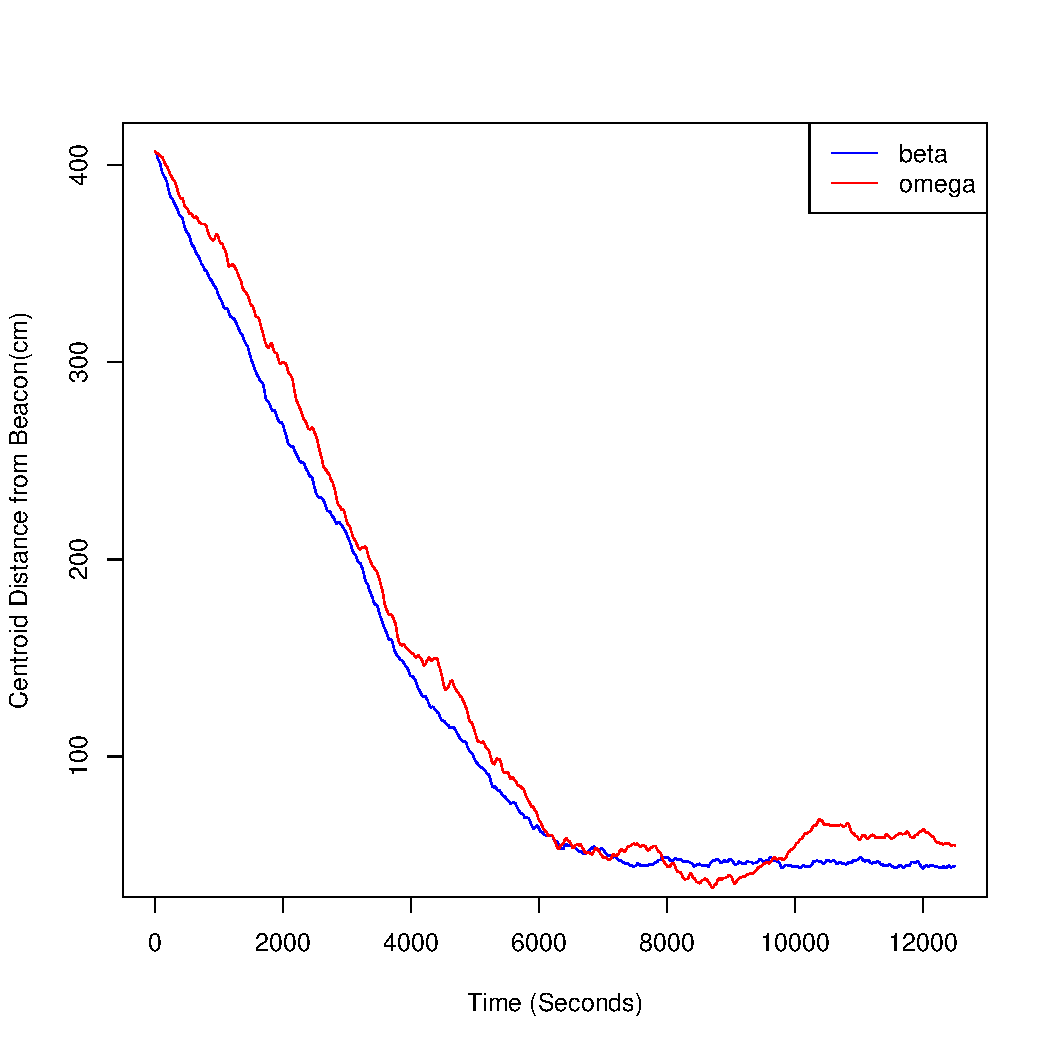
\includegraphics[width=3.5in]{figures/comparison_beacon_distance.pdf}
\caption{Distance from Beacon against Time for \textit{beta=2} and \textit{omega=35}}
\label{comparison_beacon_distance}
\end{figure}

Figure \ref{comparison_beacon_distance} plots how long each algorithm takes to reach the beacon. There is very little difference between the two algorithms with regard to this metric, they both reach the beacon at approximately the same time. The $\beta$-taxis algorithm does remain closer to the beacon after taxis has been performed but the $\omega$-taxis algorithm obtains the closest distance to the beacon. This metric does not prove that there is a significant difference between the algorithms, however it has not been measured in a particularly reliable way. It would have possibly been more correct to use a statistical test to determine significance, but as the data is time based there are few tests which are appropriate. It is simple enough to inspect the graph and see that these algorithms differ very little when measured in this way. 

In order to determine which algorithm performs best with regards to swarm aggregation the measurements of the mean distance from the swarm centroid must be compared. Unlike the previous metric, this data is not time based, as the aggregation of the swarm should remain constant throughout the experiment. In order to measure this data the Vargha-Delaney A measure will be used. This measure determines if one data set is significantly larger than the other. The result of this test when used to compare the mean distance from the swarm centroid of both data sets is 0.8958964, though there is a difference in swarm aggregation between the two algorithms it is not possible to say with 95\% confidence that is the case. 

Upon inspection of the data gathered regarding the number of lost robots, it transpired that neither algorithm ever lost any robots. This metric is therefore unable to distinguish between either of the algorithms and does not indicate that either performs more efficient taxis than the other. It is worth noting, however, that the design of the $\omega$-taxis algorithm prevents it from ever losing robots, as all robots can determine the swarm centroid no matter their location relative to it. This would suggest that the $\beta$-taxis algorithm is the superior choice here, but no valid data can be collected to prove this for these implementations.

Using the three metrics chosen it is not possible to determine that "The $\omega$-taxis algorithm performs more efficient swarm taxis than the $\beta$-taxis algorithm", rather, that the null hypothesis must be assumed, "the $\omega$-taxis algorithm and the $\beta$-taxis algorithm perform taxis at the same efficiency." However, it must be noted that very few, only twelve, simulations were performed for each algorithm due to time constraints, and the validity of these results should be questioned as a result.

\section{The Reality Gap}

The e-puck robots on which the simulator is based could be used to implement either of the algorithms described, but how well would either of them work? The $\beta$-taxis algorithm was implemented using only standard functions of the simulator, both the wireless sensor and infra-red sensors are used, both of which feature in the e-puck robots. It is important to note that the $\beta$-taxis algorithm requires the transmission of neighbour lists between robots, which is implemented in the simulator in a way not compatible with the physical robots. It would be necessary for each robot to listen for broadcasts of neighbour lists instead of querying each neighbour for the lists. 

The $\omega$-taxis algorithm is of further complication to port to real robots. Due to the way simulated robots detect the centroid of the swarm a long range infra-red sensor is required which the e-puck robots do not have. The addition of this sensor would be required in order to implement the $\omega$-taxis algorithm successfully.

\section{Conclusion}
In this paper, two swarm robotics algorithms have been implemented and tested against each other in order to determine which one is superior. Testing swarm robotics algorithms requires a vast amount of time and processing power due to the many simulation runs required in order to generate significant data. It would be wise for future research to focus on the improvement of simulation solutions available in the field of swarm robotics, as the current offerings can be difficult to use and consume large amounts of resources.

% An example of a floating figure using the graphicx package.
% Note that \label must occur AFTER (or within) \caption.
% For figures, \caption should occur after the \includegraphics.
% Note that IEEEtran v1.7 and later has special internal code that
% is designed to preserve the operation of \label within \caption
% even when the captionsoff option is in effect. However, because
% of issues like this, it may be the safest practice to put all your
% \label just after \caption rather than within \caption{}.
%
% Reminder: the "draftcls" or "draftclsnofoot", not "draft", class
% option should be used if it is desired that the figures are to be
% displayed while in draft mode.
%
%\begin{figure}[!t]
%\centering
%\includegraphics[width=2.5in]{myfigure}
% where an .eps filename suffix will be assumed under latex, 
% and a .pdf suffix will be assumed for pdflatex; or what has been declared
% via \DeclareGraphicsExtensions.
%\caption{Simulation Results}
%\label{fig_sim}
%\end{figure}

% Note that IEEE typically puts floats only at the top, even when this
% results in a large percentage of a column being occupied by floats.


% An example of a double column floating figure using two subfigures.
% (The subfig.sty package must be loaded for this to work.)
% The subfigure \label commands are set within each subfloat command, the
% \label for the overall figure must come after \caption.
% \hfil must be used as a separator to get equal spacing.
% The subfigure.sty package works much the same way, except \subfigure is
% used instead of \subfloat.
%
%\begin{figure*}[!t]
%\centerline{\subfloat[Case I]\includegraphics[width=2.5in]{subfigcase1}%
%\label{fig_first_case}}
%\hfil
%\subfloat[Case II]{\includegraphics[width=2.5in]{subfigcase2}%
%\label{fig_second_case}}}
%\caption{Simulation results}
%\label{fig_sim}
%\end{figure*}
%
% Note that often IEEE papers with subfigures do not employ subfigure
% captions (using the optional argument to \subfloat), but instead will
% reference/describe all of them (a), (b), etc., within the main caption.


% An example of a floating table. Note that, for IEEE style tables, the 
% \caption command should come BEFORE the table. Table text will default to
% \footnotesize as IEEE normally uses this smaller font for tables.
% The \label must come after \caption as always.
%
%\begin{table}[!t]
%% increase table row spacing, adjust to taste
%\renewcommand{\arraystretch}{1.3}
% if using array.sty, it might be a good idea to tweak the value of
% \extrarowheight as needed to properly center the text within the cells
%\caption{An Example of a Table}
%\label{table_example}
%\centering
%% Some packages, such as MDW tools, offer better commands for making tables
%% than the plain LaTeX2e tabular which is used here.
%\begin{tabular}{|c||c|}
%\hline
%One & Two\\
%\hline
%Three & Four\\
%\hline
%\end{tabular}
%\end{table}


% Note that IEEE does not put floats in the very first column - or typically
% anywhere on the first page for that matter. Also, in-text middle ("here")
% positioning is not used. Most IEEE journals/conferences use top floats
% exclusively. Note that, LaTeX2e, unlike IEEE journals/conferences, places
% footnotes above bottom floats. This can be corrected via the \fnbelowfloat
% command of the stfloats package.


% conference papers do not normally have an appendix


% trigger a \newpage just before the given reference
% number - used to balance the columns on the last page
% adjust value as needed - may need to be readjusted if
% the document is modified later
%\IEEEtriggeratref{8}
% The "triggered" command can be changed if desired:
%\IEEEtriggercmd{\enlargethispage{-5in}}
% references section

% can use a bibliography generated by BibTeX as a .bbl file
% BibTeX documentation can be easily obtained at:
% http://www.ctan.org/tex-archive/biblio/bibtex/contrib/doc/
% The IEEEtran BibTeX style support page is at:
% http://www.michaelshell.org/tex/ieeetran/bibtex/
%\bibliographystyle{IEEEtran}
% argument is your BibTeX string definitions and bibliography database(s)
%\bibliography{IEEEabrv,../bib/paper}
%
% <OR> manually copy in the resultant .bbl file
% set second argument of \begin to the number of references
% (used to reserve space for the reference number labels box)

\bibliographystyle{IEEEtran}
\bibliography{IEEEabrv,swin_document}




% that's all folks
\end{document}


